%%%%%%%%%%%%%%%%%%%%% {{{
%%Options for presentations (in-class) and handouts (e.g. print).
%\documentclass[pdf,9pt]{beamer}
\documentclass[pdf,9pt]{beamer}


%%%%%%%%%%%%%%%%%%%%%%
%Change this for different slides so it appears in bar
\usepackage{authoraftertitle}
\date{Chapter 6. Vector Spaces \\ \S  6-4. Finite Dimensional Spaces}

%%%%%%%%%%%%%%%%%%%%%%
%% Upload common style file
\usepackage{LyryxLAWASlidesStyle}

\begin{document}

%%%%%%%%%%%%%%%%%%%%%%%
%% Title Page and Copyright Common to All Slides

%Title Page
\input frontmatter/titlepage.tex

%LOTS Page
\input frontmatter/lyryxopentexts.tex

%Copyright Page
\input frontmatter/copyright.tex

%%%%%%%%%%%%%%%%%%%%%%%%% }}}
%-------------- start slide -------------------------------%{{{ 2

\begin{frame}[fragile]
   \tableofcontents
\end{frame}
%-------------- end slide -------------------------------%}}}
\section[\textcolor{yellow}{}]{\textcolor{yellow}{Generalizing from $\RR^n$}}
%-------------- start slide -------------------------------%{{{ 3
\frame{
\frametitle{Generalizing from $\RR^n$}
\pause
\begin{emptytitle}
    We have learnt that for a subspace $U$ of $\R^n$, if $U\neq\{\bm{0}\}$, then
    \begin{enumerate}
	\item $U$ has a basis, and $\dim(U)\leq n$.
	\item Any \textcolor{yellow}{independent subset} of $U$ can be extended (by
	    \textcolor{yellow}{adding} vectors) to a basis of $U$.
	\item Any \textcolor{yellow}{spanning set} of $U$ can be cut down (by \textcolor{yellow}{deleting} vectors) to a basis of $U$.
    \end{enumerate}
\end{emptytitle}
\vfill
\begin{center}
    \includegraphics[scale=0.015]{./figures/Section6-4-Adding.png}
    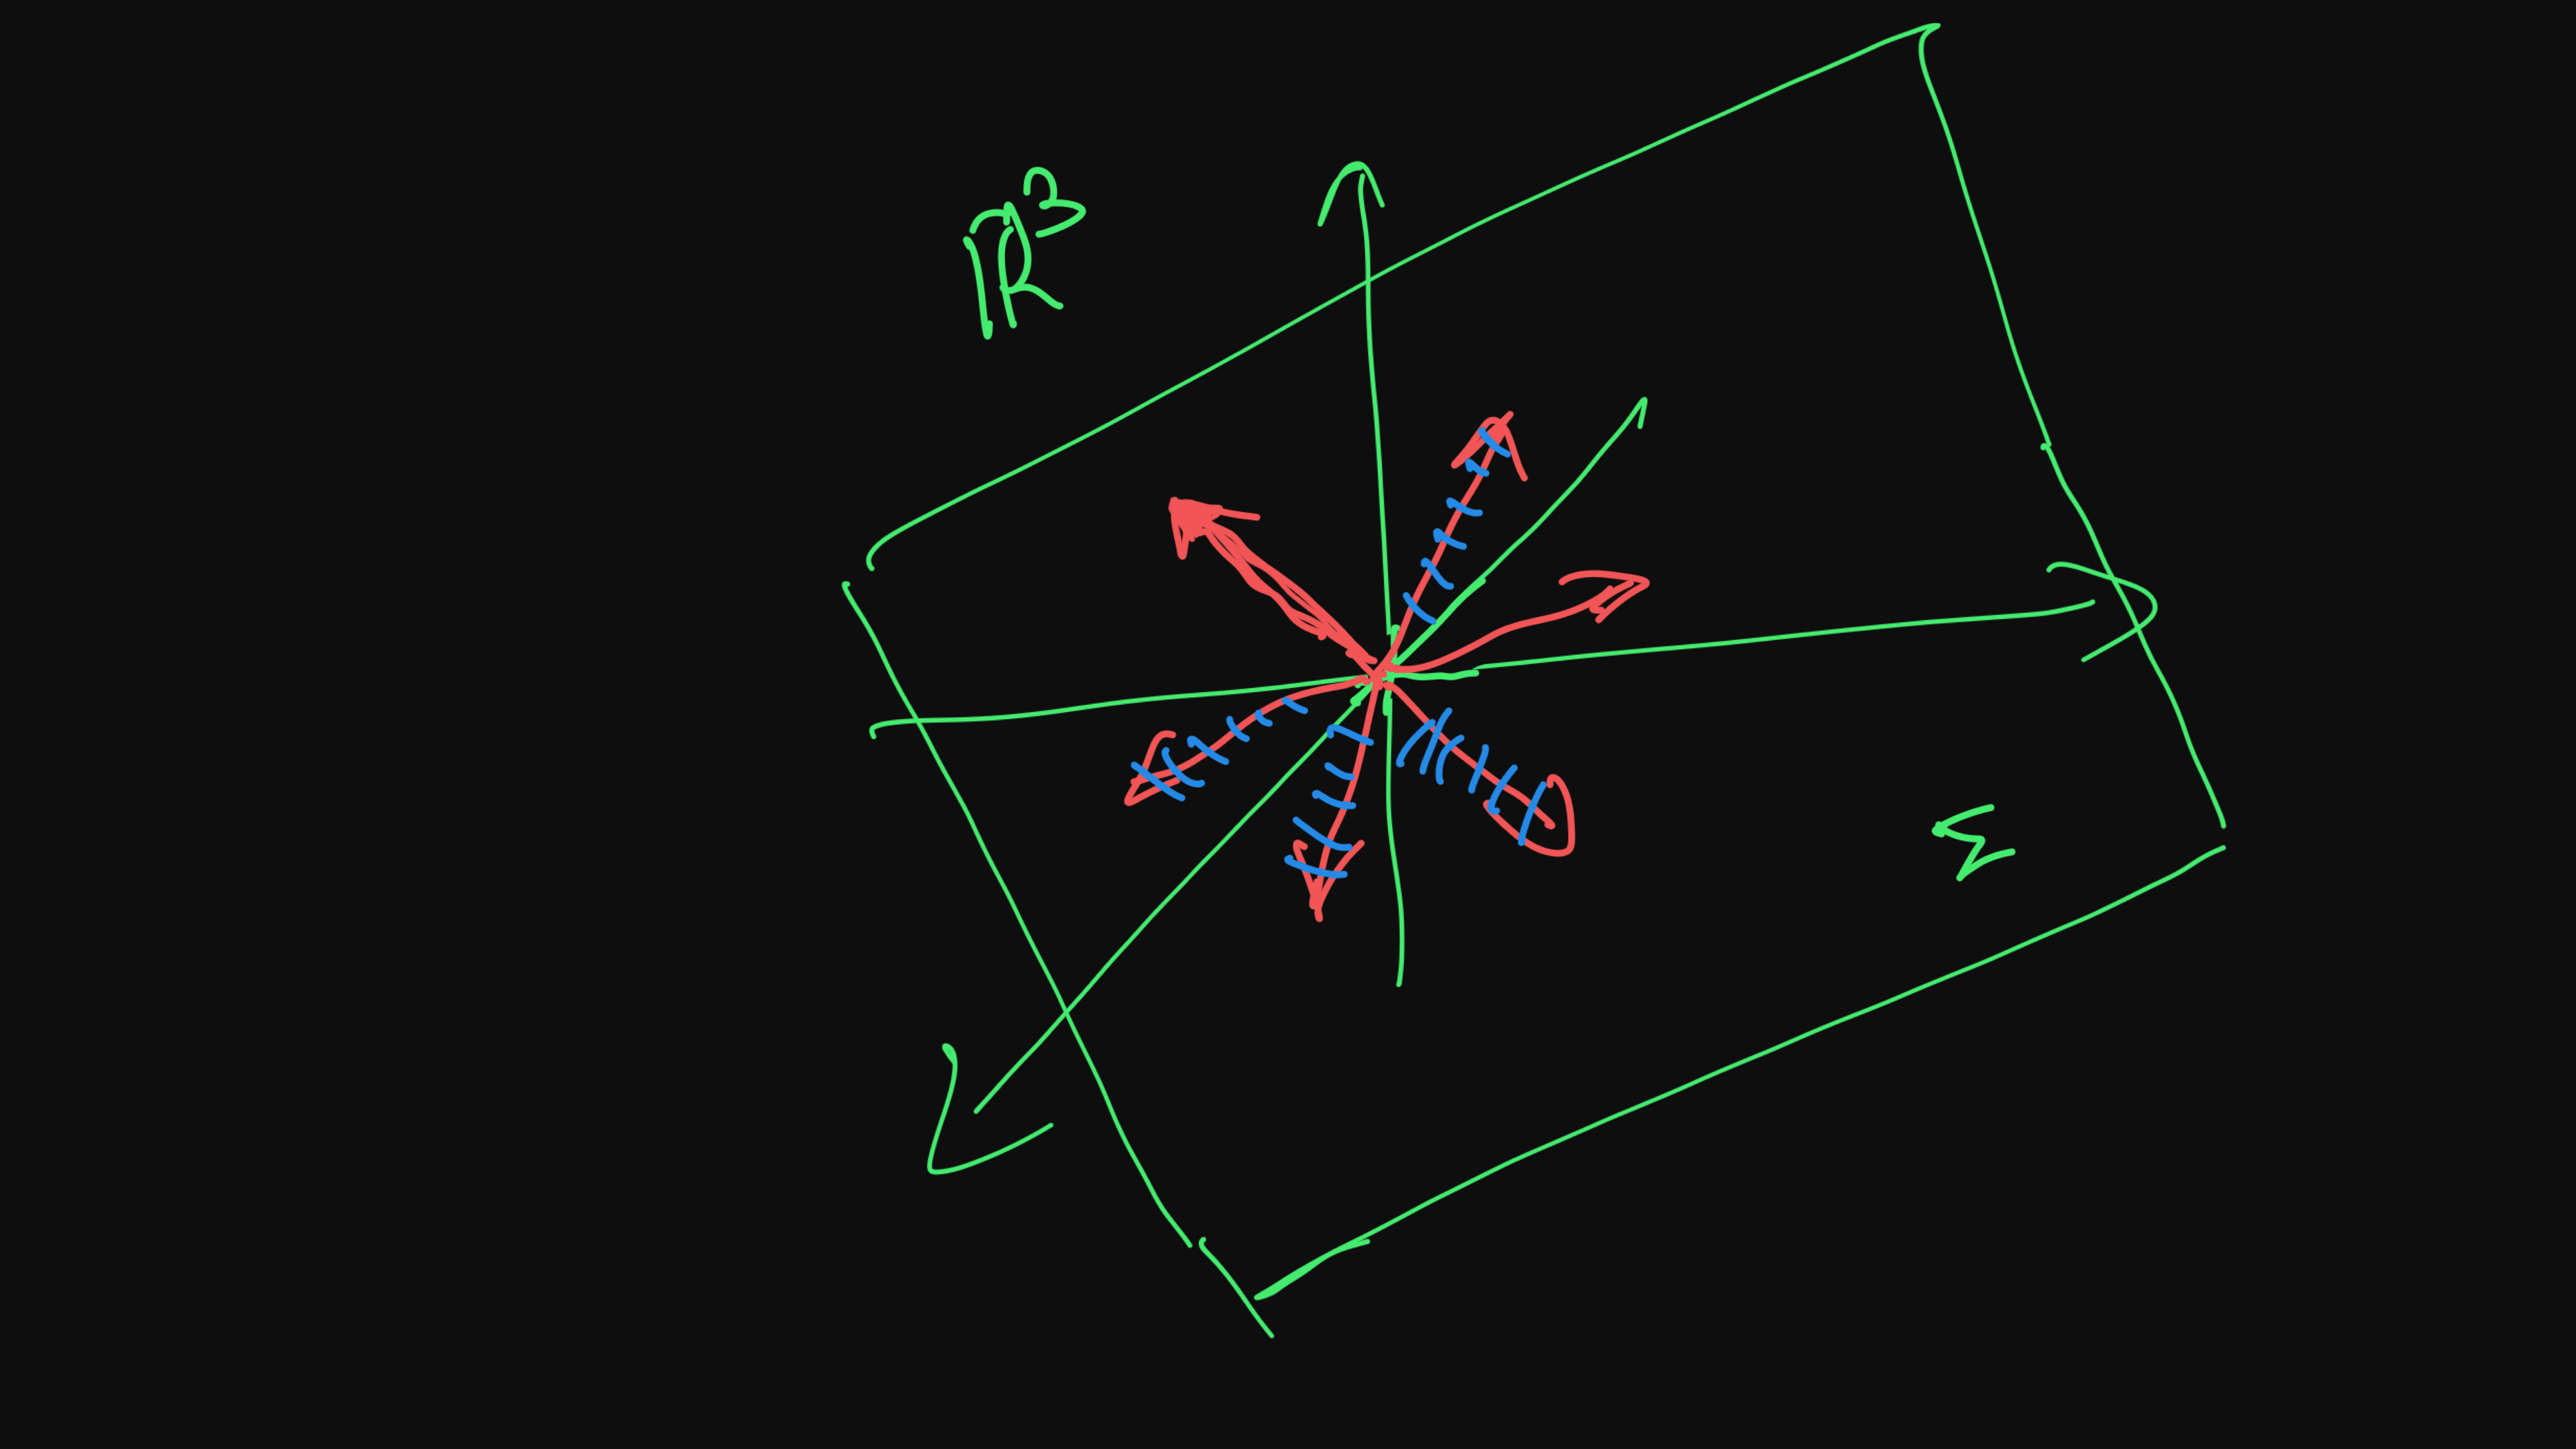
\includegraphics[scale=0.025]{./figures/Section6-4-Deleting.png}
\end{center}
}
%-------------- end slide -------------------------------%}}}
%-------------- start slide -------------------------------%{{{ 4
\frame{
\begin{definition}
    A vector space $V$ is \alert{finite dimensional} if it is
    spanned by a finite set of vectors.
    Otherwise it is called \alert{infinite dimensional}.
\end{definition}
\pause
\vfill
\begin{example}
    \begin{enumerate}
        \item $\RR^n$, ${\cal P}_n$ and $\bm{M}_{mn}$ are all examples of finite dimensional vector spaces
	\item The zero vector space, $\{ \bm{0}\}$, is also finite dimensional, since it is spanned by $\{ \bm{0}\}$.
	\item ${\cal P}$ is an infinite dimensional vector space.
    \end{enumerate}
\end{example}
}
%-------------- end slide -------------------------------%}}}
%-------------- start slide -------------------------------%{{{ 5
\frame{
\begin{lemma}[Independent Lemma]
    Let $V$ be a vector space and
    $S=\{ \bm{v}_1, \bm{v}_2, \ldots, \bm{v}_k\}$
    an independent subset of $V$.
    Suppose $\bm{u}$ is a vector in $V$. Then
    \begin{align*}
      \bm{u}\not\in\Span(S)  \quad\Longrightarrow\quad \text{$S^{\prime}=\{ \bm{v}_1, \bm{v}_2, \ldots, \bm{v}_k, \bm{u}\}$ is independent.}
    \end{align*}
\end{lemma}
\pause
\vfill
\begin{proofnoend}
    Suppose that
    $a_1\bm{v}_1 + a_2\bm{v}_2 + \cdots + a_k\bm{v}_k +a\bm{u}=\bm{0}$.
    \pause
    We claim that $a=0$. Otherwise, if $a\neq 0$, then
    \[ a\bm{u} =  -a_1\bm{v}_1 - a_2\bm{v}_2 - \cdots - a_k\bm{v}_k,\]
    implying that
    \[ \bm{u} =  -\frac{a_1}{a}\bm{v}_1 - \frac{a_2}{a}\bm{v}_2 - \cdots -
    \frac{a_k}{a}\bm{v}_k,\]
    i.e., $\bm{u}\in\Span(S)$, a contradiction.
    Therefore, $a=0$.\\ \pause
    Now $a=0$ implies that
    $a_1\bm{v}_1 + a_2\bm{v}_2 + \cdots + a_k\bm{v}_k =\bm{0}$.
    Since $S$ is independent, $a_1=a_2=\cdots=a_k=0$, and it follows that
    $S^{\prime}$ is independent.
    \myQED
\end{proofnoend}
\vfill
\begin{remark}
    Under the setting of the Independent Lemma, for $\bm{u}\in V$, we have indeed:
    \begin{align*}
	\bm{u}\not\in \Span(S) \quad\Longleftrightarrow\quad
	\text{ $S^{\prime}=\{ \bm{v}_1, \bm{v}_2, \ldots, \bm{v}_k, \bm{u}\}$ is independent.}
    \end{align*}
\end{remark}
}
%-------------- end slide -------------------------------%}}}
%-------------- start slide -------------------------------%{{{ 6
\begin{frame}[fragile]
\begin{lemma}
    Let $V$ be a finite dimensional vector space.
    If $U$ is any subspace of $V$, then any independent subset of
    $U$ can be extended to a finite basis of $U$.
\end{lemma}
\pause
\vfill
\begin{emptytitle}
\begin{center}
    \begin{minipage}{0.85\textwidth}
	\begin{algorithm*}[H]
	\SetKwInOut{Input}{Input}\SetKwInOut{Output}{Output}
	\Input{
	    1. $V$: finite dimensional vector space\\
	    2. $U\subseteq V$ a subspace\\
	    3. $W_0\subseteq U$ an independent subset of $U$
	}
	\BlankLine
	\SetAlgoLined
	 $W_0\to W$\;
	 \While{$\Span\{W\}\ne U$}{
	   Pick up arbitrary $\bm{x}\in U\setminus \Span\{W\}$\;
	   $\{\bm{x}\}  \cup W \to W$\;
	   Independent Lemma guarantees that the new $W$ is an independent set\;
	 }
	 \Output{$W$, that is independent and spans $U$; hence a basis of $U$. }
	 \caption{Proof of Lemma}
	\end{algorithm*}
    \end{minipage}
\end{center}
    % The proof of this lemma involves repeated application of the
    % {\bf Independent Lemma},
    % and then the {\bf Fundamental Theorem.}
\end{emptytitle}
\end{frame}
%-------------- end slide -------------------------------%}}}
\section[\textcolor{yellow}{}]{\textcolor{yellow}{Constructing basis from independent sets by \alert{adding} vectors}}
%-------------- start slide -------------------------------%{{{ 7
\frame{
\frametitle{Constructing basis from independent sets by \alert{adding} vectors}
\pause
\begin{theorem}
    Let $V$ be a finite dimensional vector space spanned by a set
    of $m$ vectors.
    \begin{enumerate}[(1)]
	\item $V$ has a finite basis, and $\dim(V) \leq m$.
	    \pause
	\item Every independent subset of $V$ can be extended to a
	    basis of $V$ \alert{by adding vectors from any fixed basis
	    of $V$}.
	    \pause
	\item If $U$ is a subspace of $V$, then\\
	    (i) $U$ is finite dimensional and $\dim(U)\leq\dim(V)$;\\
	    (ii) every basis of $U$ is part of a basis of $V$.
    \end{enumerate}
\end{theorem}
\vfill
\pause
\begin{proofnoend}
    (1) If $V=\{\bm{0}\}$, then $V$ has dimension zero, and the (unique) basis of $V$ is the empty
    set.  Otherwise, choose any nonzero vector $\bm{x}$ in $V$ and extend $\{\bm{x}\}$ to a finite
    basis $B$ of $V$ (by a previous {\bf Lemma}).  By the {\bf Fundamental Theorem}, $B$ has at most
    $m$ elements, so $\dim(V)\leq m$.
\end{proofnoend}
}
%-------------- end slide -------------------------------%}}}
%-------------- start slide -------------------------------%{{{ 8
\begin{frame}[fragile]
    \begin{proofnoend}
	(2)
	\begin{center}
	\begin{minipage}{0.98\textwidth}
	    \begin{algorithm*}[H]
	    \SetKwInOut{Input}{Input}\SetKwInOut{Output}{Output}
	    \Input{
		1. $V$: finite dimensional vector space spanned by $m$ vectors\\
		2. $B$: a basis of $V$ (exists by part (1))\\
		3. $W_0$: an independent set of vectors in $V$
	    }
	    \BlankLine
	    \SetAlgoLined
	     $W_0\to W$\;
	     \While{$\Span \{W\}\ne V$}{
		 Find out one $\bm{x}\in B\setminus \Span\{W\}$\;
	       $\{\bm{x}\}  \cup W \to W$\;
	       Independent Lemma guarantees that the new $W$ is an independent set\;
	     }
	     \Output{$W$, that is independent and spans $V$; hence a basis of $V$. }
	     \caption{Proof of part 2}
	    \end{algorithm*}
	\end{minipage}
	\end{center}% Repeat.
    \end{proofnoend}
\end{frame}
%-------------- end slide -------------------------------%}}}
%-------------- start slide -------------------------------%{{{ 9
\begin{frame}[fragile]
\begin{proofnoend}
    (3-i)
    If $U=\{\bm{0}\}$, then $\dim(U)=0\leq m=\dim(V)$.
    Otherwise, choose $\bm{x}$ to be any nonzero vector of $U$ and
    extend $\{\bm{x}\}$ to a basis $B$ of $U$ (again by a previous {\bf Lemma}).
    Since $B$ is an independent subset of $V$, $B$ has at most $\dim(V)$
    elements, so $\dim(U)\leq\dim(V)$.\\
    \pause
    \bigskip

    (3-ii)
    If $U=\{\bm{0}\}$, then any basis of $V$ suffices.
    Otherwise, any basis $B$ of $U$ can be extended to a basis
    of $V$:
    because $B$ is independent, we apply part (2) of this theorem.
    \myQED
\end{proofnoend}
\end{frame}
%-------------- end slide -------------------------------%}}}
%-------------- start slide -------------------------------%{{{ 10
\frame{
\begin{problem}
    Extend the independent set
    $S=\left\{
	\left[\begin{array}{r} 1 \\ -1 \\ 1 \\ -1 \end{array}\right],
	\left[\begin{array}{r} 2 \\ 3  \\ 4 \\ 5  \end{array}\right]\right\}$
    to a basis of $\RR^4$.
\end{problem}
\pause
\vfill
\begin{solution}[method 1.]
    Let $A=\left[\begin{array}{rrrr}
    1 & -1 & 1 & -1 \\ 2 & 3 & 4 & 5 \end{array}\right]$.
    Because the elementary row operations won't change row space, let's find
    the reduced row-echelon form of $A$
    \[
	R = \left[\begin{array}{rrrr}
		1 & 0 & 7/5 & 2/5 \\
		0 & 1 & 2/5 & 7/5
	    \end{array}\right].
    \]
    ($\row(A)=\row(R)$.)
    We need add two rows to $R$ to get a nonsingular matrix:
    \[
	    \left[\begin{array}{cccc}
		1 & 0 & 7/5 & 2/5 \\
		0 & 1 & 2/5 & 7/5 \\
		* & * & *   & *   \\
		* & * & *   & *   \\
	    \end{array}\right]
    \]
\end{solution}
}
%-------------- end slide -------------------------------%}}}
%-------------- start slide -------------------------------%{{{ 11
\frame{
\begin{solution}[continued]
    There are certainly multiple choices for those two rows. The simplest choice might be the following:
    \[
	    \left[\begin{array}{cc|cc}
		1 & 0 & 7/5 & 2/5 \\
		0 & 1 & 2/5 & 7/5 \\ \hline
		0 & 0 & 1   & 0   \\
		0 & 0 & 0   & 1   \\
	    \end{array}\right]
    \]
    Hence,
    \[ B=\left\{
        \left[\begin{array}{r} 1 \\ -1 \\ 1 \\ -1 \end{array}\right],
        \left[\begin{array}{r} 2 \\ 3 \\ 4 \\ 5 \end{array}\right],
	\vec{e}_3, \vec{e}_4 \right\},
    \]
    gives a basis for $\R^4$.
    % we have that $\Span \{B\} \subseteq \R^4$. Moreover, $\dim(\Span \{B\} ) = 4 = \dim(\R^4)$, by Part (3-i) of theorem,
    % $\Span \{B\}=\R^4 $. Finally, because vectors in $B$ are independent, $B$ is a basis for $\R^4$.
    \myQED
\end{solution}
}
%-------------- end slide -------------------------------%}}}
%--------------ostart slide -------------------------------%{{{ 12
\begin{frame}[fragile]
    \begin{emptytitle}
    Below is a more systematical way to find all possible choices based on one basis from $V$
    \end{emptytitle}
    \vfill
    \begin{solution}[method 2.]
	\begin{align*}
	    A= \left[\begin{array}{cc|cccc}
		1  & 2 & 1 & 0 & 0 & 0 \\
		-1 & 3 & 0 & 1 & 0 & 0 \\
		1  & 4 & 0 & 0 & 1 & 0 \\
		-1 & 5 & 0 & 0 & 0 & 1 \\
	    \end{array}\right]
	    \to
	    R = \left[\begin{array}{cc|cccc}
		1 & 2 & 1            & 0            & 0 & 0 \\
		0 & 1 & \frac{1}{5}  & \frac{1}{5}  & 0 & 0 \\
		0 & 0 & -\frac{7}{5} & -\frac{2}{5} & 1 & 0 \\
		0 & 0 & -\frac{2}{5} & -\frac{7}{5} & 0 & 1 \\
	    \end{array}\right]
	\end{align*}
	Now we need to find four columns which include the first two columns from the six
	columns of $R$ to form a nonsingular matrix. Then the corresponding columns from $A$ form a basis for $\R^4$.
	Indeed, we can choose any two columns from the last four columns.
	If we choose the last two columns, this will give the result from the previous answer.
	\myQED
    \end{solution}
\end{frame}
%-------------- end slide -------------------------------%}}}
%-------------- start slide -------------------------------%{{{ 13
\frame{
\begin{problem}
    Extend the independent set $S=\{x^2-3x+1, 2x^3+3\}$ to a basis of ${\cal P}_3$.
\end{problem}
\pause
\vfill
\begin{solution}[method 1.]
    Using the fact that polynomials of distinct orders are independent, we need only include missing
    orders. Hence:
    $B= \{\textcolor{yellow}{1},\textcolor{yellow}{x}, x^2-3x+1, 2x^3+3\}$.
    \myQED
\end{solution}
\vfill
\pause
\begin{remark}
   What happens if $S= \{x^2-3x +1, 2x^2 +3\}$?
\end{remark}
}
%-------------- end slide -------------------------------%}}}
%-------------- start slide -------------------------------%{{{ 14
\begin{frame}[fragile]
    \begin{solution}[method 2.]
	Transform each vector -- polynomial -- to a row vector and form a matrix:
	\begin{align*}
	    A = \begin{pmatrix}
		    1 & -3 & 1 & 0 \\
		    3 & 0  & 0 & 2 \\
		\end{pmatrix}
	\end{align*}
	Now the question is how one can add two rows to $A$ to make it nonsingular:
	\begin{align*}
	    \begin{pmatrix}
		1 & -3 & 1 & 0 \\
		3 & 0  & 0 & 2 \\
		* & *  & * & * \\
		* & *  & * & * \\
	    \end{pmatrix}
	\end{align*}
	It is ready to check that the last two rows to be any of the following:
	\begin{align*}
	    \begin{pmatrix}
		1 & 0 & 0 & 0 \\
		0 & 1 & 0 & 0 \\
	    \end{pmatrix}\quad\text{or}\quad
	\begin{pmatrix}
		1 & 0 & 0 & 0 \\
		0 & 0 & 1 & 0 \\
	    \end{pmatrix}\quad\text{or}\quad
	\begin{pmatrix}
		0 & 0 & 1 & 0 \\
		0 & 0 & 0 & 1 \\
	    \end{pmatrix}\quad\text{or}\quad ...
	\end{align*}
	For example, if we choose make the first choice, this will give us $\{1,x\}$ as the
	additional two polynomials. Therefore, we obtain a basis:
	$B= \{\textcolor{yellow}{1},\textcolor{yellow}{x}, x^2-3x+1, 2x^3+3\}.$
	\myQED
    \end{solution}
    \pause
    \vfill
    \begin{solution}[method 3.]
       Carry out columns-wise... \myQED
    \end{solution}
\end{frame}
%-------------- end slide -------------------------------%}}}
%-------------- start slide -------------------------------%{{{ 15
\frame{
\begin{problem}
Extend the independent set
\[ S=\left\{
	\left[\begin{array}{rr} -1 & 1 \\ 0  & 0 \end{array}\right],
	\left[\begin{array}{rr} 1  & 0 \\ -1 & 0 \end{array}\right],
	\left[\begin{array}{rr} 0  & 1 \\ 0  & 1 \end{array}\right]\right\}\]
to a basis of $\bm{M}_{22}$.
\end{problem}
\pause
\vfill
\begin{solution}
    $S$ can be extended to a basis of $\bm{M}_{22}$ by adding a matrix
    from the standard basis of $\bm{M}_{22}$.
    To methodically find such a matrix, try to express each matrix
    of the standard basis of $\bm{M}_{22}$ as a linear combination
    of the matrices of $S$.
    This results in four systems of linear equations, each in three
    variables, and these can be solved simultaneously by putting the
    augmented matrix in row-echelon form.
    \[
	\left[\begin{array}{rrr|rrrr}
		-1 & 1  & 0 & 1 & 0 & 0 & 0 \\
		1  & 0  & 1 & 0 & 1 & 0 & 0 \\
		0  & -1 & 0 & 0 & 0 & 1 & 0 \\
		0  & 0  & 1 & 0 & 0 & 0 & 1
	\end{array}\right]
	\rightarrow
	\left[\begin{array}{rrr|rrrr}
		1 & -1 & 0 & -1 & 0  & 0  & 0 \\
		0 & 1  & 1 & 1  & 1  & 0  & 0 \\
		0 & 0  & 1 & 1  & 1  & 1  & 0 \\
		0 & 0  & 0 & -1 & -1 & -1 & 1
	\end{array}\right].
    \]
\end{solution}
}
%-------------- end slide -------------------------------%}}}
%-------------- start slide -------------------------------%{{{ 16
\frame{
\begin{solution}[continued]
    The row-echelon matrix indicates that all four systems
    are inconsistent, and thus any of the four matrices in the
    standard basis of $\bm{M}_{22}$ can be used to extend $S$
    to an independent subset of four vectors (matrices) of $\bm{M}_{22}$.
    Let
    \[ B=\left\{
	\left[\begin{array}{rr} -1 & 1 \\ 0  & 0 \end{array}\right],
	\left[\begin{array}{rr} 1  & 0 \\ -1 & 0 \end{array}\right],
	\left[\begin{array}{rr} 0  & 1 \\ 0  & 1 \end{array}\right],
	\left[\begin{array}{rr} 1  & 0 \\ 0  & 0 \end{array}\right]\right\}.\]

    If $\Span(B)\neq {\bm M}_{22}$, then apply the {\bf Independent Lemma}
     to get an independent set with five vectors
    (matrices).
    Since ${\bm M}_{22}$ is spanned by
    \[ \left\{
	\left[\begin{array}{rr} 1 & 0 \\ 0 & 0 \end{array}\right],
	\left[\begin{array}{rr} 0 & 1 \\ 0 & 0 \end{array}\right],
	\left[\begin{array}{rr} 0 & 0 \\ 1 & 0 \end{array}\right],
	\left[\begin{array}{rr} 0 & 0 \\ 0 & 1 \end{array}\right]\right\},\]
    this contradicts the {\bf Fundamental Theorem}.
    Therefore $\Span(B)=\bm{M}_{22}$, and $B$
    is a basis of $\bm{M}_{22}$.
    \myQED
\end{solution}
}
%-------------- end slide -------------------------------%}}}
\section[\textcolor{yellow}{}]{\textcolor{yellow}{Subspaces of finite dimensional vector spaces}}
%-------------- start slide -------------------------------%{{{ 17
\frame{
\frametitle{Subspaces of finite dimensional vector spaces}
\pause
\begin{theorem}
    Let $V$ be a finite dimensional vector space,
    and let $U$ and $W$ be subspaces of $V$.
    \begin{enumerate}
	\item If $U\subseteq W$, then $\dim(U)\leq\dim(W)$.
	\item If $U\subseteq W$ and $\dim(U)=\dim(W)$, then $U=W$.
    \end{enumerate}
\end{theorem}
\pause
\vfill
\begin{emptytitle}
    This is the generalization to finite dimensional vector spaces
    of the corresponding result for $\RR^n$.
\end{emptytitle}
\pause
\vfill
\begin{proofnoend}
    \begin{enumerate}
	\item
	    Since $W$ is a subspace of a finite dimensional vector space,
	    this result follows from a previous  {\bf Theorem}.

	\item
	    Let $B$ be a basis of $U$, and suppose $|B|=k=\dim(W)$.
	    Since $U\subseteq W$, $B$ is an independent subset
	    of $W$.
	    If $\Span(B)\neq W$, then $W$ contains an independent
	    set of size $k+1$, contradicting the {\bf Fundamental Theorem}.
	    Therefore, $B$ is a basis of $W$, and thus $U=W$.

	    %If $\dim(U)=\dim(W)=k$, then $U$ has a basis $B$ of size $k$.
	    %Since $U\subseteq W$, $B$ is an independent subset of $W$
	    %having size $k$, and thus can be extended to a basis of $W$.
	    %However, if this basis contains vectors other than those
	    %of $B$, then $\dim(U)\neq\dim(W)$, a contradiction.
	    %Therefore, $B$ is a basis of $W$, and thus $U=W$.
	    %\vspace*{-.26in}
    \end{enumerate}
\myQED    \end{proofnoend}
}
%-------------- end slide -------------------------------%}}}
%-------------- start slide -------------------------------%{{{ 18
\frame{
\begin{problem}
    Let $a\in\RR$ be fixed, and let
    \[ U=\{ p(x)\in{\cal P}_n ~|~ p(a)=0\}.\]
    Then $U$ is a subspace of ${\cal P}_n$ (you should be able
    to prove this).
    Show that
    \[ S=\{ (x-a), (x-a)^2, (x-a)^3, \ldots, (x-a)^n\}\]
    is a basis of $U$.
\end{problem}
\pause
\vfill
\begin{remark}[Hints of the proof]
    We need to show that the following:
    \begin{enumerate}
	\item Show that $\Span(S)\subseteq U$, and that $S$ is independent.
	\item Deduce that $n\leq \dim(U) \leq n+1$.
	\item Show that $\dim(U)$ can not equal $n+1$.
    \end{enumerate}
\end{remark}
}
%-------------- end slide -------------------------------%}}}
%-------------- start slide -------------------------------%{{{ 19
\frame{
\begin{solution}
    \begin{itemize}
	\item Each polynomial in $S$ has $a$ as a root, so $S\subseteq U$.  Since
	    $U$ is a subspace of ${\cal P}_n$ it follows that  $\Span(S)\subseteq
	    U$.
	\item Since the polynomials in $S$ have distinct degrees ($(x-a)^i$ has
	    degree $i$), $S$ is independent.  \item Since $\Span(S)\subseteq
	    U\subseteq {\cal P}_n$, it follows that
	    \[ \dim(\Span(S))\leq \dim(U)\leq \dim({\cal P}_n).\]
	    Since $S$ is a basis of $\Span(S)$, $\dim(\Span(S))=n$;
	    also, $\dim({\cal P}_n)=n+1$, and thus
	    $n\leq \dim(U)\leq n+1$.
	\item Finally, if $\dim(U)=n+1$, then $U={\cal P}_n$, implying that every
	    polynomial in ${\cal P}_n$ has $a$ as a root.  However, $x-a+1\in{\cal
	    P}_n$ but  $x-a+1\not\in U$, so $\dim(U)\neq n+1$.  Therefore,
	    $\dim(U)=n$.
    \end{itemize}
    We now have $\Span(S)\subseteq U$ and $\dim(\Span(S))=n=\dim(U)$.
    By a previous {\bf Theorem}, $U=\Span(S)$, and hence $S$ is a basis
    of $U$.
    \myQED
\end{solution}
}
%-------------- end slide -------------------------------%}}}
\section[\textcolor{yellow}{}]{\textcolor{yellow}{Constructing basis from spanning sets by \alert{deleting} vectors}}
%-------------- start slide -------------------------------%{{{ 20
\frame{
\begin{lemma}[Dependent Lemma]
    Let $V$ be a vector space and
    $D=\{ \bm{v}_1, \bm{v}_2,\ldots,\bm{v}_k\}$ a subset of $V$,
    $k\geq 2$.
    Then $D$ is dependent if and only if there is some vector
    in $D$ that is a linear combination of the other vectors in $D$.
\end{lemma}
\pause
\vfill
\begin{proofnoend}
    ``$\Rightarrow$" Suppose that $D$ is dependent.
    Then
    \[ t_1\bm{v}_1 +t_2\bm{v}_2 +\cdots +t_k\bm{v}_k=\bm{0}\]
    for some $t_1, t_2, \ldots, t_k\in \RR$ not all equal to zero.
    Note that we may assume that $t_1\neq 0$.
    Then
    \begin{eqnarray*}
	t_1\bm{v}_1 & = & -t_2\bm{v}_2 - t_3\bm{v}_3 -\cdots -t_k\bm{v}_k \\
	\bm{v}_1    & = & -\frac{t_2}{t_1}\bm{v}_2 -\frac{t_3}{t_1}\bm{v}_3 -\cdots -\frac{t_k}{t_1}\bm{v}_k;
    \end{eqnarray*}
    i.e., $\bm{v}_1$ is a linear combination of $\bm{v}_2, \bm{v}_3, \ldots, \bm{v}_k$.
\end{proofnoend}
}
%-------------- end slide -------------------------------%}}}
%-------------- start slide -------------------------------%{{{ 21
\frame{
\begin{proofnoend}[continued]
    ``$\Leftarrow$" Conversely, assume that some vector in $D$ is a linear combination of
    the other vectors of $D$.
    We may assume that $\bm{v}_1$ is a linear combination of
    $\bm{v}_2, \bm{v}_3, \ldots, \bm{v}_k$.
    Then
    \[\bm{v}_1 = s_2\bm{v}_2 + s_3\bm{v}_3 +\cdots +s_k\bm{v}_k \]
    for some $s_2, s_3, \ldots, s_k\in\RR$, implying that
    \[1\bm{v}_1 - s_2\bm{v}_2 - s_3\bm{v}_3 -\cdots -x_k\bm{v}_k = \bm{0}. \]
    Thus there is a nontrivial linear combination of the vectors of $D$
    that vanishes, so $D$ is dependent.
    \myQED
\end{proofnoend}
\pause
\vfill
\begin{emptytitle}
    Suppose $U=\Span(S)$ for some set of vectors $S$.
    If $S$ is dependent, then we can find a vector $\bm{v}$
    in $S$ that is a linear combination of the other vectors
    of $S$.
    Deleting $\bm{v}$ from $S$ results if a set $T$ with
    $\Span(T)=\Span(S)=U$.
\end{emptytitle}
}
%-------------- end slide -------------------------------%}}}
%-------------- start slide -------------------------------%{{{ 22
\frame{
\frametitle{Constructing basis from spanning sets by \alert{deleting} vectors}
\pause
\begin{theorem}
    Let $V$ be a finite dimensional vector space.
    Then any spanning set $S$ of $V$ can be cut down to a basis of
    $V$ by deleting vectors of $S$.
\end{theorem}
\pause
\vfill
\begin{proofnoend}
\begin{center}
    \begin{minipage}{0.98\textwidth}
	\begin{algorithm*}[H]
	\SetKwInOut{Input}{Input}\SetKwInOut{Output}{Output}
	\Input{
	    1. $V$: finite dimensional vector space spanned by $m$ vectors\\
	    3. $S$: a spanning set of $V$
	}
	\BlankLine
	\SetAlgoLined
	 $S \to W$\;
	 \While{$W$ is dependent}{
	     Find out one $\bm{x}\in W$ that can be linearly represented by the rest\;
	   $W \setminus \{\bm{x}\} \to W$\;
	   Dependent Lemma guarantees that the span of the new $W$ remains to be $V$\; 
	 }
	 \Output{$W$, that is independent and spans $V$; hence a basis of $V$. }
	 \caption{Proof of Theorem}
	\end{algorithm*}
    \end{minipage}
    \myQED
\end{center}
\end{proofnoend}
}
%-------------- end slide -------------------------------%}}}
%-------------- start slide -------------------------------%{{{ 23
\frame{
\begin{problem}
    Let
    \[
	X_1=\left[\begin{array}{rr} 1  & 1 \\ 1  & -1 \end{array}\right], \quad
	X_2=\left[\begin{array}{rr} 2  & 0 \\ -2 & 1 \end{array}\right], \quad
	X_3=\left[\begin{array}{rr} -1 & 1 \\ 0  & -2 \end{array}\right],\]
    \[
	X_4=\left[\begin{array}{rr} 1 & 2 \\ -1 & 1 \end{array}\right],\quad\text{and}\quad
	X_5=\left[\begin{array}{rr} 0 & 2 \\ 2  & -3 \end{array}\right],\]
	and let $U=\{ X_1, X_2, X_3, X_4, X_5 \}$.
    Then $\Span(U)=\bm{M}_{22}$.
    Find a basis of $\bm{M}_{22}$ from among the elements of $U$.
\end{problem}
\pause
\vfill
\begin{solution}
    Since $U$ has five matrices and $\dim(\bm{M}_{22})=4$, $U$ is dependent.
    Suppose
    \[ aX_1 +bX_2+cX_3+dX_4+eX_5=\bm{0}_{22}.\]
    This gives us a homogeneous system of four equations in
    five variables, whose general solution is
    \[ a=-\frac{4}{3}t;\quad b=\frac{1}{3}t;\quad c=-\frac{2}{3}t;\quad d=0;\quad e=t, \quad \mbox{ for } t\in\RR.\]
\end{solution}
}
%-------------- end slide -------------------------------%}}}
%-------------- start slide -------------------------------%{{{ 24
\frame{
\begin{solution}[continued]
    Taking $t=3$ gives us
    \[ -4X_1 +X_2-2X_3+3X_5=\bm{0}_{22}.\]
    From this, we see that $X_1$ can be expressed as a linear
    combination of $X_2$, $X_3$ and $X_5$.
    %(similarly, $X_2$ can be written as a linear combination of
    %$X_1$, $X_3$ and $X_5$;
    %$X_3$ can be written as a linear combination of
    %$X_1$, $X_2$ and $X_5$;
    %$X_5$ can be written as a linear combination of
    %$X_1$, $X_2$ and $X_3$).
    \medskip

    Let
    \[ B=\{ X_2, X_3, X_4, X_5\}.\]
    Then $\Span(B)=\Span(U)=\bm{M}_{22}$.
    If $B$ is not independent, then apply the {\bf Dependent Lemma}
    to find a subset of three matrices of $B$ that spans $\bm{M}_{22}$.
    Since
    \[ \left\{
    \left[\begin{array}{rr} 1 & 0 \\ 0 & 0 \end{array}\right],
    \left[\begin{array}{rr} 0 & 1 \\ 0 & 0 \end{array}\right],
    \left[\begin{array}{rr} 0 & 0 \\ 1 & 0 \end{array}\right],
    \left[\begin{array}{rr} 0 & 0 \\ 0 & 1 \end{array}\right]\right\}\]
    is an independent subset of $\bm{M}_{22}$, this contradicts the
    {\bf Fundamental Theorem}.
    Therefore $B$ is independent, and hence is a basis of $\bm{M}_{22}$.
    \myQED
\end{solution}
}
%-------------- end slide -------------------------------%}}}
%-------------- start slide -------------------------------%{{{ 25
\frame{
\begin{theorem}[Generalization of $\R^n$]
    Let $V$ be a finite dimensional vector space with $\dim(V)=n$,
    and suppose $S$ is a subset of $V$ containing $n$ vectors.
    Then $S$ is independent if and only if $S$ spans $V$.
\end{theorem}
\pause
\vfill
\begin{proofnoend}
    $(\Rightarrow)$
    Suppose $S$ is independent.
    Since every independent set of $V$
    can be extended to a basis of $V$, there exists a basis $B$ of $V$ with
    $S\subseteq B$.
    However, $|S|=n$ and $|B|=n$, and therefore $S=B$, i.e., $S$ is
    a basis of $V$.
    In particular, this implies that $S$ spans $V$.
    \medskip
    \pause

    $(\Leftarrow)$
    Conversely, suppose that $\Span(S)=V$.
    Since every spanning set of $V$ can be cut down to a basis of $V$,
    there exists a basis $B$ of $V$ with $B\subseteq S$.
    However, $|S|=n$ and $|B|=n$, and therefore $S=B$, i.e., $S$ is
    a basis of $V$.
    In particular, this implies that $S$ is an independent set of $V$.
    \myQED
\end{proofnoend}
\pause
\vfill
\begin{remark}
    This theorem can be used to simplify the arguments used in various problems covered.
\end{remark}
}
%-------------- end slide -------------------------------%}}}
%-------------- start slide -------------------------------%{{{ 26
\frame{
    \begin{problem}
	Find a basis of ${\cal P}_2$ among the elements of the set
	\[ U = \left\{
	x^2-3x+2,\quad 1-2x,\quad 2x^2+1,\quad 2x^2-x-3\right\}.\]
    \end{problem}
    \pause
    \begin{solution}
	Since $|U|=4>3=\dim({\cal P}_2)$, $U$ is dependent.
	\medskip

	Suppose
	$a(x^2-3x+2)+b(1-2x)+c(2x^2+1)+d(2x^2-x-3)=0$; then
	\[ (a+2c+2d)x^2+(-3a-2b-d)x+(2a+b+c-3d)=0.\]
	This leads to a system of three equations in four variables that
	can be solved using gaussian elimination.
	\[ \left[\begin{array}{rrrr|r}
		1  & 0  & 2 & 2  & 0 \\
		-3 & -2 & 0 & -1 & 0 \\
		2  & 1  & 1 & -3 & 0
	    \end{array}\right]
	\rightarrow
	\left[\begin{array}{rrrr|r}
		1 & 0 & 2  & 0 & 0 \\
		0 & 1 & -3 & 0 & 0 \\
		0 & 0 & 0  & 1 & 0
	    \end{array}\right] \]
	Thus $a=-2t$, $b=3t$, $c=t$ and $d=0$ for any $t\in\RR$.
	Also, since each row of the reduced row-echelon matrix has
	a leading one, $U$ spans ${\cal P}_2$.
    \end{solution}
}
%-------------- end slide -------------------------------%}}}
%-------------- start slide -------------------------------%{{{ 27
\frame{
\begin{solution}[continued]
    Let $t=-1$.
    Then
    \[ 2(x^2-3x+2)-3(1-2x)-(2x^2+1)=0,\]
    so any one of $\left\{ x^2-3x+2, 1-2x, 2x^2+1\right\}$ can be
    expressed as a linear combination of the other two.
    Let's remove $x^2-3x+2$. Hence, set
    \[ B=\left\{1-2x, 2x^2+1, 2x^2-x-3 \right\}.\]
    Then $\Span(B)=\Span(U)={\cal P}_2$.
    Since $|B|=3=\dim({\cal P}_2)$, it follows from
     that $B$ is independent.
    Therefore, $B\subseteq U$ is a basis of ${\cal P}_2$.
    \myQED
\end{solution}
}
%-------------- end slide -------------------------------%}}}
%-------------- start slide -------------------------------%{{{ 28
\frame{
\begin{problem}
    Let $V=\{ A\in\bm{M}_{22} ~|~ A^T = A\}$.
    Then $V$ is a vector space.
    Find a basis of $V$ consisting of
    \alert{invertible} matrices.
\end{problem}
\pause
\vfill
\begin{remark}
    Note that $V$ is the set of $2\times 2$ symmetric matrices,
    so
    \[ V=\left\{\left.\left[\begin{array}{cc} a & b \\ b & c \end{array}\right]
    ~\right|~ a,b,c\in\RR\right\}
    =\Span\left\{
	\left[\begin{array}{cc} 1 & 0 \\ 0 & 0 \end{array}\right],
	\left[\begin{array}{cc} 0 & 1 \\ 1 & 0 \end{array}\right],
	\left[\begin{array}{cc} 0 & 0 \\ 0 & 1 \end{array}\right]
    \right\}  \]
    From this, we deduce that $\dim(V)=3$. \alert{(Why?)}
    Thus,
    a basis of $V$ consisting of invertible matrices
    will consist of \alert{three independent symmetric invertible matrices.}
\end{remark}
}
%-------------- end slide -------------------------------%}}}
%-------------- start slide -------------------------------%{{{ 29
\frame{
\begin{solution}
    There are many solutions.
    Let
    \[
	A= \left[\begin{array}{cc} 1 & 0 \\ 0 & 0 \end{array}\right], \quad
	B= \left[\begin{array}{cc} 0 & 1 \\ 1 & 0 \end{array}\right], \quad
	C= \left[\begin{array}{cc} 0 & 0 \\ 0 & 1 \end{array}\right].\]
    The matrix $B$ is invertible, so one approach is to take
    linear combinations of $A$ and $C$ to produce two independent
    invertible matrices; for example
    \[
	A+C=\left[\begin{array}{cc} 1 & 0 \\ 0 & 1 \end{array}\right]\quad\text{and}\quad
	A-C=\left[\begin{array}{cc} 1 & 0 \\ 0 & -1 \end{array}\right].\]
    It is easy to verify that $S=\{ A+C, A-C, B\}$ is an independent
    subset of $2\times 2$ invertible symmetric matrices.
    Since $|S|=3=\dim(V)$, $S$ spans $V$ and is therefore a basis of $V$.
    \myQED
\end{solution}
}
%-------------- end slide -------------------------------%}}}
\section[\textcolor{yellow}{}]{\textcolor{yellow}{Sums and Intersections}}
%-------------- start slide -------------------------------%{{{ 30
\frame{
\frametitle{Sums and Intersections}
\pause
\vfill
\begin{definition}
    Let $V$ be a vector space, and let $U$ and $W$ be subspaces of $V$.
    Then
    \begin{enumerate}
	\item $U+W = \{ \bm{u+w} ~|~ \bm{u}\in U\quad\text{and}\quad \bm{w}\in W\}$ and is
	    called the \alert{sum} of $U$ and $W$.
	    \pause
	\item $U\cap W = \{ \bm{v} ~|~ \bm{v}\in U\quad\text{and}\quad \bm{v}\in W\}$ and is
	    called the \alert{intersection} of $U$ and $W$.
	\item If $U$ and $W$ are subspaces of a vector space $V$ and
	    $U\cap W=\{\bm{0}\}$, then the sum of $U$ and $W$ is call the
	    \alert{direct sum} and is denoted $U\oplus W$.
    \end{enumerate}
\end{definition}
\vfill
\pause
\begin{lemma}
    Prove that both $U+W$ and $U\cap W$ are subspaces of $V$.
\end{lemma}
}
%-------------- end slide -------------------------------%}}}
%-------------- start slide -------------------------------%{{{ 31
\frame{
\begin{proofnoend}[of $U+W$]
    \begin{enumerate}
	\item Since $U$ and $W$ are subspaces of $V$, ${\bm 0}$, the zero
	    vector of $V$, is an element of both $U$ and $W$.
	    Since ${\bm 0}+{\bm 0}={\bm 0}$, ${\bm 0}\in U+W$.
	\item Let $\bm{x}_1, \bm{x}_2\in U + W$.
	    Then $\bm{x}_1=\bm{u}_1+\bm{w}_1$ and
	    $\bm{x}_2=\bm{u}_2+\bm{w}_2$ for some $\bm{u}_1,\bm{u}_2\in U$ and
	    $\bm{w}_1,\bm{w}_2\in W$.
	    It follows that
	    \[ \bm{x}_1 + \bm{x}_2 = (\bm{u}_1+\bm{w}_1) + (\bm{u}_2+\bm{w}_2)
	    = (\bm{u}_1+\bm{u}_2) + (\bm{w}_1+\bm{w}_2).\]
	    Since $U$ and $W$ are subspaces of $V$, $\bm{u}_1+\bm{u}_2\in U$
	    and $\bm{w}_1+\bm{w}_2\in W$, and therefore $\bm{x}_1 + \bm{x}_2\in U+W$.
	\item Let $\bm{x}_1\in U + W$ and $k\in\RR$.
	    Then $\bm{x}_1=\bm{u}_1+\bm{w}_1$ for some $\bm{u}_1\in U$ and
	    $\bm{w}_1\in W$.
	    It follows that
	    $k\bm{x}_1 = k(\bm{u}_1+\bm{w}_1)
	     =  (k\bm{u}_1)+(k\bm{w}_1)$.
	    Since $U$ and $W$ are subspaces of $V$, $k\bm{u}_1\in U$
	    and $k\bm{w}_1\in W$, and therefore $k\bm{x}_1\in U+W$.
    \end{enumerate}
    By the {\em Subspace Test}, $U+W$ is a subspace of $V$.
    \myQED
\end{proofnoend}

}
%-------------- end slide -------------------------------%}}}
%-------------- start slide -------------------------------%{{{ 32
\frame{
\begin{theorem}
    If $U$ and $W$ are finite dimensional subspaces of
    a vector space $V$, then $U+W$ is finite dimensional and
    \[ \dim(U+W) = \dim(U) + \dim(W) -\dim(U\cap W).\]
\end{theorem}
\vfill
\begin{remark}
    $V$ need not be finite dimensional!
\end{remark}
}
%-------------- end slide -------------------------------%}}}
%-------------- start slide -------------------------------%{{{ 33
\begin{frame}[fragile]
    \begin{center}
	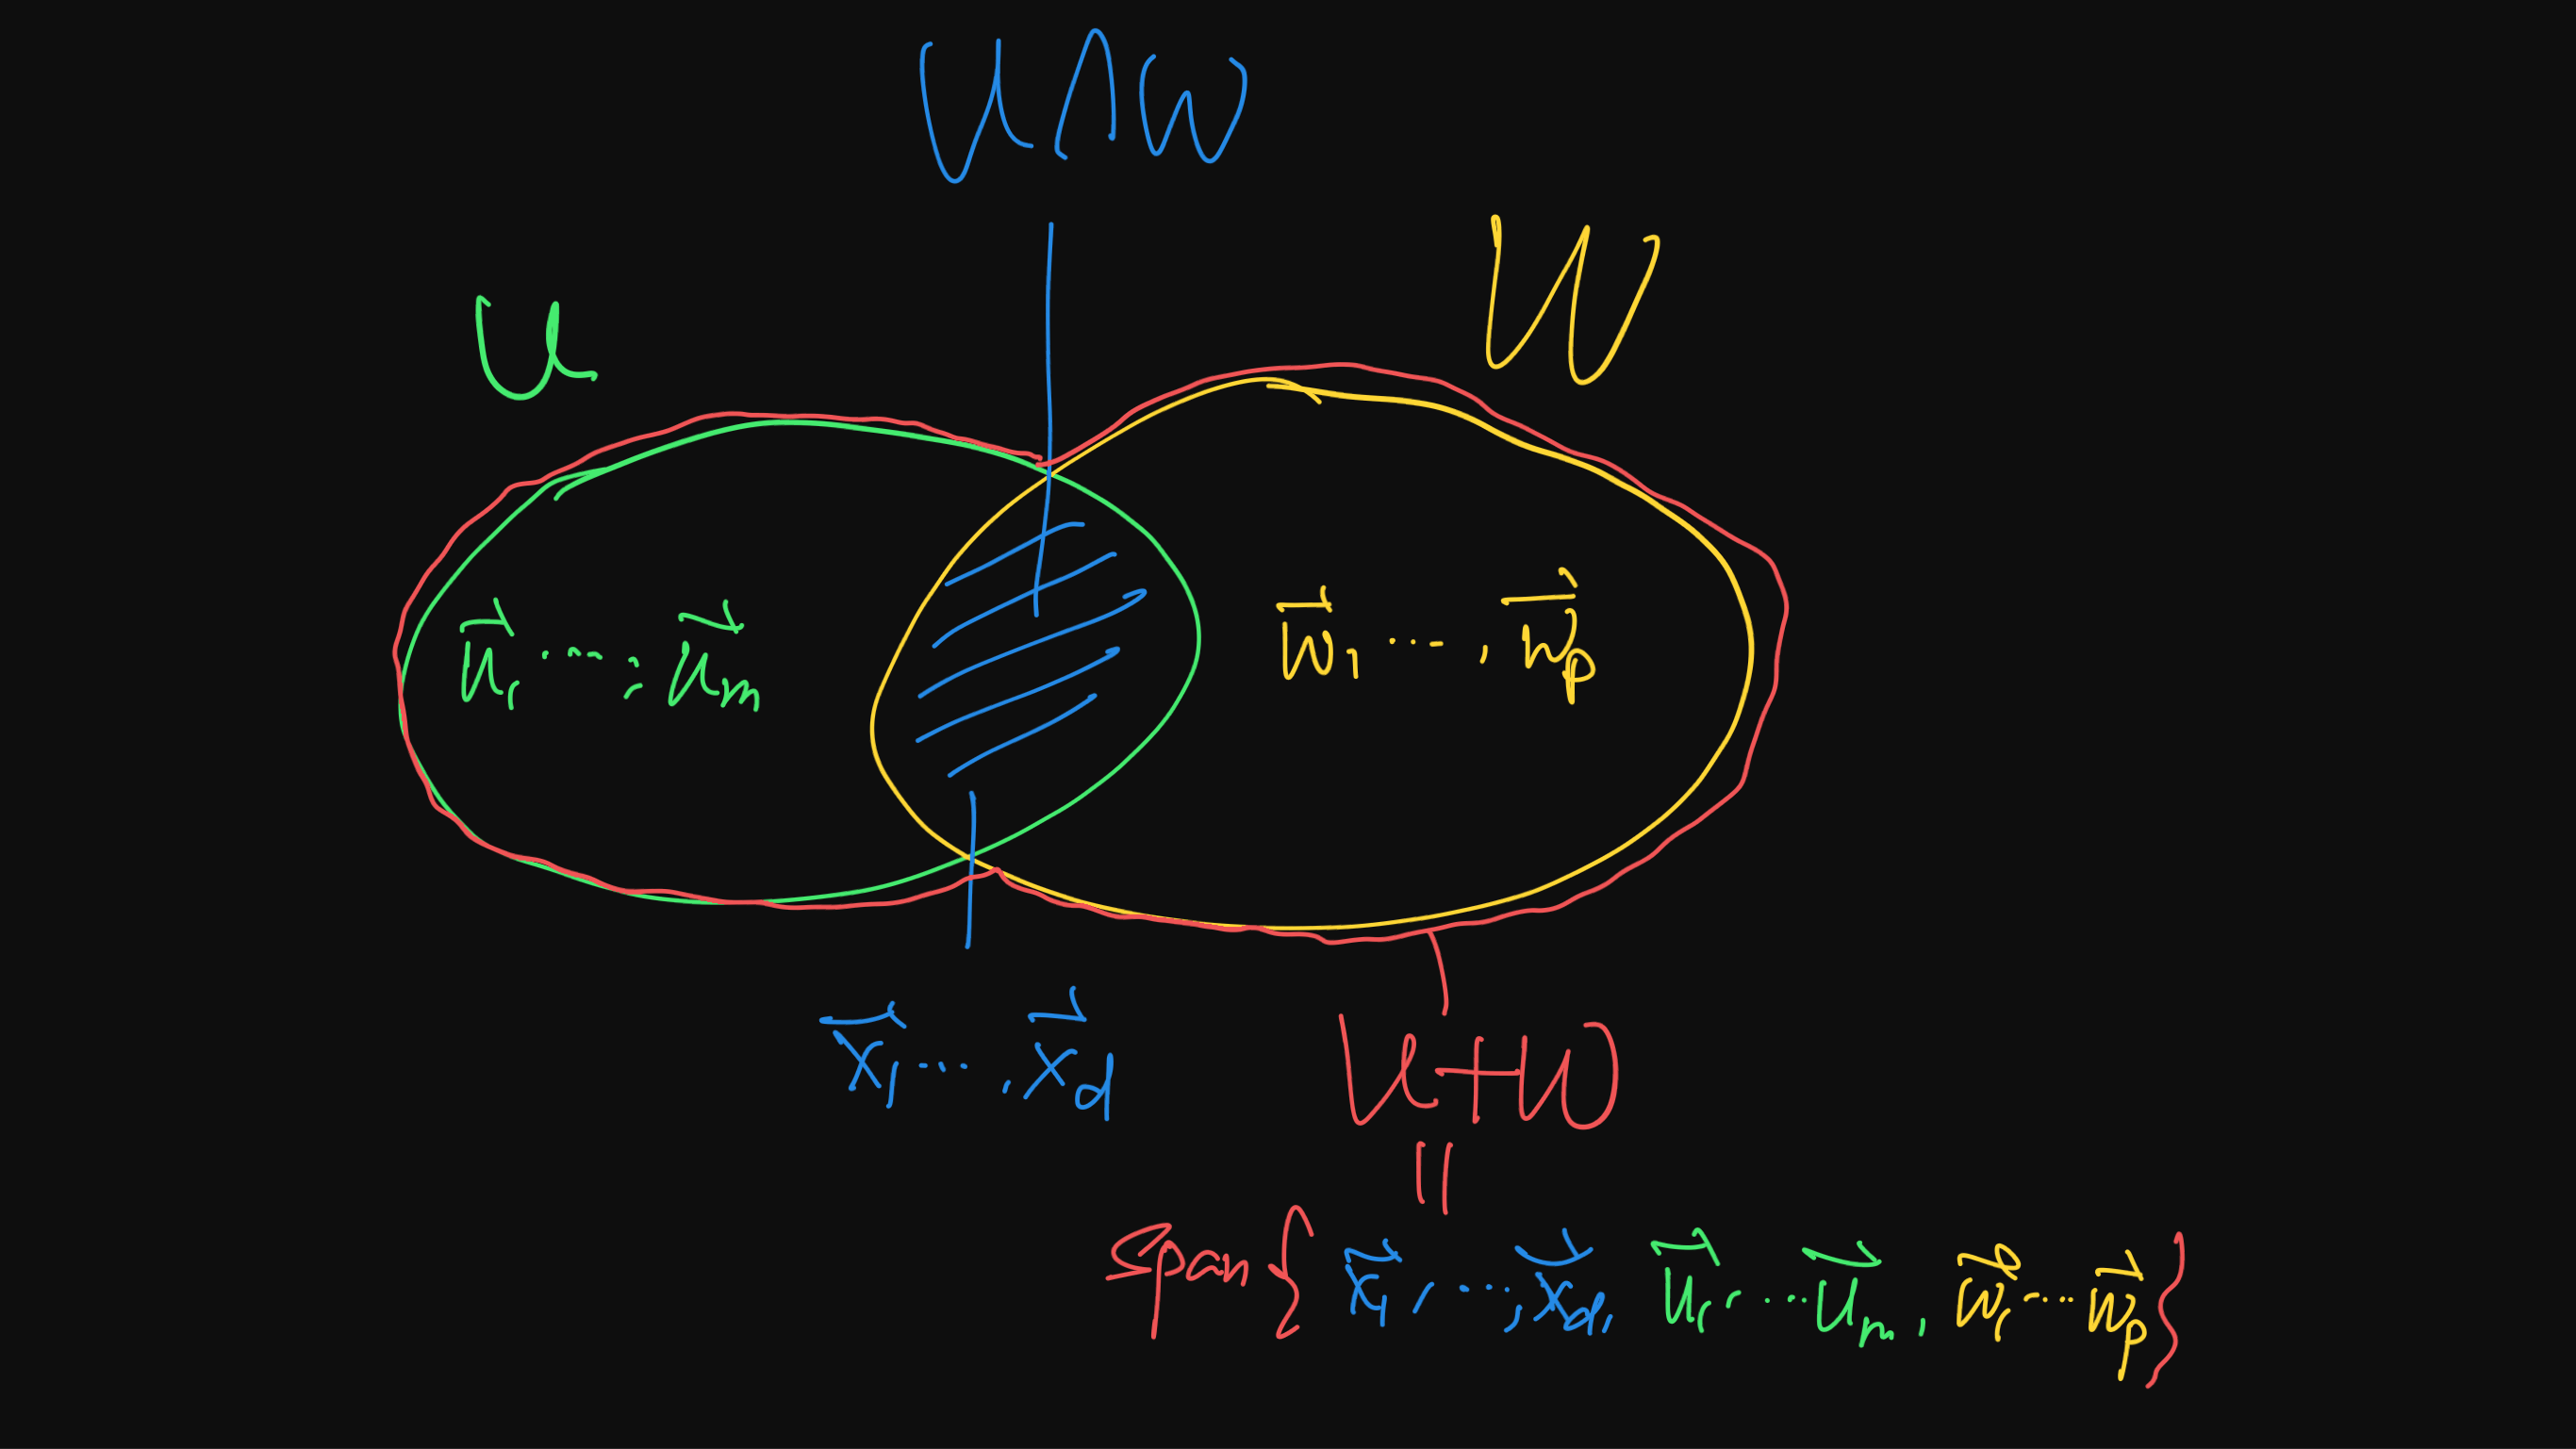
\includegraphics[scale=0.07]{./figures/Thm6-5-4.png}
    \end{center}
    \vspace{-2em}
    \begin{proofnoend}
	$U\cap W$ is a subspace of the finite dimensional vector space $U$, so
	is finite dimensional, and has a finite basis
	$X=\{ \bm{x}_1, \bm{x}_2, \ldots, \bm{x}_d\}$.
	Since $X\subseteq U\cap W$, $X$ can be extended to a finite basis
	$B_U$ of $U$ and a finite basis $B_W$ of $W$:
	\[
	    B_U=\{ \bm{x}_1, \bm{x}_2, \ldots, \bm{x}_d,
	    \bm{u}_1, \bm{u}_2, \ldots, \bm{u}_m \}
	    \quad\text{and}\quad
	    B_W=\{ \bm{x}_1, \bm{x}_2, \ldots, \bm{x}_d,
	    \bm{w}_1, \bm{w}_2, \ldots, \bm{w}_n \}.
	\]
	Then
	\begin{align*}
	    \Span \left\{ \bm{x}_1,\cdots \bm{x}_d,\bm{u}_1,\cdots,\bm{u}_m,\bm{w}_1,\cdots,\bm{w}_p\right\} = U+W.
	\end{align*}
    \end{proofnoend}
\end{frame}
%-------------- end slide -------------------------------%}}}
%-------------- start slide -------------------------------%{{{ 34
\begin{frame}[fragile]
    \begin{proofnoend}[continued]
	What remains is to prove that
	\[ B=\{ \bm{x}_1, \bm{x}_2, \ldots, \bm{x}_d,
		\bm{u}_1, \bm{u}_2, \ldots, \bm{u}_m,
	\bm{w}_1, \bm{w}_2, \ldots, \bm{w}_n \}\]
	is a basis of $U+W$ since then it implies that
	\[ \dim(U+W) = \dim(U) + \dim(W) -\dim(U\cap W)\]
	\[\Updownarrow\]
	\[ d+m+p = (d+m) + (d+p) - d \]
\end{proofnoend}
\end{frame}
%-------------- end slide -------------------------------%}}}
%-------------- start slide -------------------------------%{{{ 34
\begin{frame}[fragile]
    \begin{proofnoend}[continued]
	To prove $B$ is linearly independent, we need to show that
	\begin{align*}
	    r_1 \bm{x}_1 + \cdots + r_d\bm{x}_d +
	    s_1 \bm{u}_1 + \cdots + s_m\bm{u}_m +
	    t_1 \bm{w}_1 + \cdots + t_p\bm{w}_p  = \bm{0}.
	\end{align*}
	which is equivalent to
	\begin{align*}
	    \underbrace{r_1 \bm{x}_1 + \cdots + r_d\bm{x}_d +
	    s_1 \bm{u}_1 + \cdots + s_m\bm{u}_m }_{\in U} =
	    \underbrace{- t_1 \bm{w}_1 - \cdots - t_p\bm{w}_p}_{\in W}
	\end{align*}
	Hence,
	\begin{enumerate}
	    \item $LHS\in  U\cap W$, which implies that $s_1=\cdots = s_m=0$.
	    \item $RHS\in  U\cap W$, which implies that $t_1=\cdots = t_p=0$.
	\end{enumerate}
	Finally,
	\begin{align*}
	    r_1 \bm{x}_1 + \cdots + r_d\bm{x}_d =\bm{0}
	\end{align*}
	implies that $r_1=\cdots =r_d=0$.
	This proves that $B$ is independent.
	\myQED
\end{proofnoend}
\end{frame}
%-------------- end slide -------------------------------%}}}
\end{document}
